%%%%%%%%%%%%%%%%%%%%%%% file template.tex %%%%%%%%%%%%%%%%%%%%%%%%%
%
% This is a general template file for the LaTeX package SVJour3
% for Springer journals.          Springer Heidelberg 2010/09/16
%
% Copy it to a new file with a new name and use it as the basis
% for your article. Delete % signs as needed.
%
% This template includes a few options for different layouts and
% content for various journals. Please consult a previous issue of
% your journal as needed.
%
%%%%%%%%%%%%%%%%%%%%%%%%%%%%%%%%%%%%%%%%%%%%%%%%%%%%%%%%%%%%%%%%%%%
%
% First comes an example EPS file -- just ignore it and
% proceed on the \documentclass line
% your LaTeX will extract the file if required
\begin{filecontents*}{example.eps}
%!PS-Adobe-3.0 EPSF-3.0
%%BoundingBox: 19 19 221 221
%%CreationDate: Mon Sep 29 1997
%%Creator: programmed by hand (JK)
%%EndComments
gsave
newpath
  20 20 moveto
  20 220 lineto
  220 220 lineto
  220 20 lineto
closepath
2 setlinewidth
gsave
  .4 setgray fill
grestore
stroke
grestore
\end{filecontents*}
%
\RequirePackage{fix-cm}
%
%\documentclass{svjour3}                     % onecolumn (standard format)
%\documentclass[smallcondensed]{svjour3}     % onecolumn (ditto)
\documentclass[smallextended]{svjour3}       % onecolumn (second format)
%\documentclass[twocolumn]{svjour3}          % twocolumn
%
\smartqed  % flush right qed marks, e.g. at end of proof
%
\usepackage{graphicx}
\usepackage{code}
%
% \usepackage{mathptmx}      % use Times fonts if available on your TeX system
%
% insert here the call for the packages your document requires
%\usepackage{latexsym}
% etc.
%
% please place your own definitions here and don't use \def but
% \newcommand{}{}
%
% Insert the name of "your journal" with
\journalname{International Journal on Software Tools for Technology Transfer}
%
\begin{document}

\title{TSTL: The Template Scripting Testing Language}

%\subtitle{Do you have a subtitle?\\ If so, write it here}

%\titlerunning{Short form of title}        % if too long for running head

\author{Josie Holmes \and
Alex Groce \and
Jervis Pinto \and
Pranjal Mittal \and
Pooria Azimi \and
James O'Brien
}

%\authorrunning{Short form of author list} % if too long for running head

\institute{F. Author \at
              first address \\
              Tel.: +123-45-678910\\
              Fax: +123-45-678910\\
              \email{fauthor@example.com}           %  \\
%             \emph{Present address:} of F. Author  %  if needed
           \and
           S. Author \at
              second address
}

\date{Received: date / Accepted: date}
% The correct dates will be entered by the editor


\maketitle

\begin{abstract}
Test case reduction has long been seen as essential to effective automated testing.  However, test case reduction simply reduces the \emph{length} of a test case.  It does not attempt to reduce \emph{semantic} complexity.  This paper presents algorithms for normalizing and generalizing test cases.  Rewriting test cases into a \emph{normal form} can reduce semantic complexity and, often, remove steps from an already delta-debugged test case.  Normalization, more importantly, reduces the \emph{number} of test cases that a reader must examine, partially addressing the ``fuzzer taming'' problem of discovering all faults in a large set of failing test cases.  Generalization, in contrast, takes a test case and reports what aspects of the test could have been changed while preserving the property that the test fails.  These algorithms rely on the features of a recently introduced domain-specific language, TSTL.  Normalization plus generalization aids understanding of test cases, including tests for TSTL itself and for complex and widely used Python APIs such as the NumPy numeric computation library and the ArcPy GIS scripting package.  Normalization frequently reduces the number of test cases to be examined by \emph{over an order of magnitude}, and often to just one test case per fault.  Together, ideally, normalization and generalization allow a user to replace reading a large set of test cases that vary in unimportant ways with reading \emph{one annotated test case, summarizing an entire family of similar failures}.
\keywords{Software testing \and Domain-specific languages \and
  Explicit-state model checking \and End-user testing}
% \PACS{PACS code1 \and PACS code2 \and more}
% \subclass{MSC code1 \and MSC code2 \and more}
\end{abstract}

\section{Introduction}

It has long been understood that effective automated testing requires
test case reduction \cite{DD,MinUnit,ICSEDiff} to produce test cases
that remove irrelevant operations.  In fact, test case reduction is
now standard practice in industral testing tools such as Mozilla's
{\tt jsfunfuzz}.  However, simply reducing the length of a test case
does not produce any kind of semantic simplicity.  There may be many
1-minimal test cases that present different variations of a single
fault.  In many cases, reading more than one of these test cases
provides no useful additional information on the cause of failure.

Consider the three test cases shown in Figure \ref{threetests}.  These
test cases are obviously very similar, and in fact all lead to a
violation of the property that an AVL tree must always be nearly
balanced, due to a missing call to {\tt rebalance} in {\tt delete} in
a Python implementation of AVL trees.  However, the test cases are
syntactically very different, and a testing system that collects
failing test cases will produce three tests for a user to examine.
While there are methods for attempting to determine which test cases
represent distinct faults \cite{PLDI13}, the ideal solution is
arguably to rewrite all three of these test cases into a single,
normal form that preserves the structure of the failure while removing
such accidental aspects of each test case as the particular integer
values and variables used, and the ordering of assignments and
insertions.

Figure \ref{normalgen} shows the result of applying our \emph{test case
  normalization} method to these three tests, and then applying our
\emph{test case generalization} approach to the normalized test case.
\emph{All three test cases normalize to the same test
case}.  This single test case, in addition to the 10 steps required to produce
the failure, includes comments indicating what about the test case can
be changed while still failing in the same way.  For instance, the
value 1 assigned to {\tt int0} in step 0 is not essential.  It could
be changed to any value in the range 5-20 (the total set of values
allowed by the test generator) without changing the final result.  The
same is true of the assignment of 3 to {\tt int1}.  Similarly, the
exact ordering of many steps in the test case is not important.  Finally,
step 9 is annotated to show that instead of using the existing value
of {\tt int1} (4), a fresh assignment could be inserted before the
{\tt delete} call, setting {\tt
  int1} to 3 instead.  These possible
changes are not meant to be combined --- the annotation claims only
that changing these aspects of the test case one at a time will
preserve failure.

Combining normalization and generalization avoids some common problems
with understanding automatically generated test cases.  For instance,
when a large integer appears in such a test case, the question always
arises --- is this unusual value important, or just a randomly chosen
number of no significance \cite{MakeMost}?  After normalization, any
large values in a test case are sure to be essential, rather than
accidental, because normalization includes value minimization.
Without the additional step of generalization, however, it would be
easy to conclude that \emph{all} small numeric values in normalized tests are
accidental.  Generalization informs a user when a small value is
required to reproduce a failure, and when it is simply an artifact of normalization.

Normalization is not a complete solution to the problem of
identifying distinct faults (one key limitation is that our algorithms do not apply to
complex custom test generators such as CSmith \cite{csmith} or {\tt
  jsfunfuzz} \cite{jsfunfuzz}), but it is highly effective when it applies,
in our experience.
Running 100,000 tests (of length 100) on the faulty AVL tree produces
860 failing test cases with no duplicates.  Normalizing these reduces
the number of distinct failing test cases to only 22.  Of course,
ideally \emph{all} failures due to the same fault would normalize to a
single, representative test case, but we can only aim to approximate
such a canonical form for faults.  Figure \ref{diffnorm} shows a test
case that normalizes differently, and its normalized form (we omit the
generalization, which is not interestingly different than that for the
first normalized test case).

The contributions of this paper are 1) the idea of normalizing and
generalizing test cases, 2) algorithms for normalizing and
generalizing test cases that make use of the abstract graph interface
for testing provided by the TSTL \cite{NFM15,ISSTA15} testing
language, and 3) some initial experimental results showing the value
of test case normalization and generalization.  We show that
normalization and generalization has been key to efforts to understand
complex failing test cases for a widely-used, highly complex library
for GIS automation.

\begin{figure}
{\scriptsize
{\bf Test case \#1}
\begin{code}
avl0 = avl.AVLTree() 
int0 = 4 
int2 = 13 
int3 = 7 
avl0.insert(int2) 
avl0.insert(int3) 
int1 = 15 
avl0.insert(int1) 
avl0.insert(int0) 
avl0.delete(int2)
\end{code}
{\bf Test case \#2}
\begin{code}
int0 = 14 
avl0 = avl.AVLTree() 
int2 = 13 
int1 = 15 
avl0.insert(int1) 
int1 = 11 
avl0.insert(int2) 
avl0.insert(int0) 
avl0.insert(int1) 
avl0.delete(int0) 
\end{code}
{\bf Test case \#3}
\begin{code}
avl1 = avl.AVLTree() 
int3 = 18 
avl1.insert(int3) 
int0 = 5 
int3 = 12 
avl1.insert(int0) 
int0 = 15 
avl1.insert(int0) 
avl1.insert(int3) 
int1 = 15 
avl1.delete(int1) 
\end{code}
}
\caption {Three randomly generated test cases for the same fault.}
\label{threetests}
\end{figure}

\begin{figure}
{\scriptsize
\begin{code}
\textcolor{black!35}{\#[}
int0 = 1                              \textcolor{black!35}{\# STEP 0}
\textcolor{black!35}{\#  or int0 = 5 }
\textcolor{black!35}{\#   - int0 = 20} 
\textcolor{black!35}{\#  swaps with step 4}
int1 = 3                              \textcolor{black!35}{\# STEP 1}
\textcolor{black!35}{\#  or int1 = 5 }
\textcolor{black!35}{\#   - int1 = 20} 
\textcolor{black!35}{\#  swaps with step 6}
avl0 = avl.AVLTree()                  \textcolor{black!35}{\# STEP 2}
\textcolor{black!35}{\#] (steps in [] can be in any order)}
avl0.insert(int0)                     \textcolor{black!35}{\# STEP 3}
\textcolor{black!35}{\#[}
int0 = 2                              \textcolor{black!35}{\# STEP 4}
\textcolor{black!35}{\#  swaps with step 0}
avl0.insert(int1)                     \textcolor{black!35}{\# STEP 5}
\textcolor{black!35}{\#] (steps in [] can be in any order)}
int1 = 4                              \textcolor{black!35}{\# STEP 6}
\textcolor{black!35}{\#  or int1 = 5 }
\textcolor{black!35}{\#   - int1 = 20} 
\textcolor{black!35}{\#  swaps with step 1}
avl0.insert(int1)                     \textcolor{black!35}{\# STEP 7}
avl0.insert(int0)                     \textcolor{black!35}{\# STEP 8}
avl0.delete(int1)                     \textcolor{black!35}{\# STEP 9}
\textcolor{black!35}{\#  or (}
\textcolor{black!35}{\#      int1 = 3  ;}
\textcolor{black!35}{\#      avl0.delete(int1) }
\textcolor{black!35}{\#     )}
\end{code}
}
\caption{Normalization and generalization for all three test cases.
  Lines beginning with \# are comments in Python, used for annotations.}
\label{normalgen}
\end{figure}

\begin{figure}
{\scriptsize
{\bf Test case \#4:}
\begin{code}
int0 = 10 
int2 = 7 
avl1 = avl.AVLTree() 
avl1.insert(int2) 
avl1.insert(int0) 
int1 = 1 
int3 = 1 
avl1.insert(int3) 
int3 = 15 
avl1.insert(int3) 
avl1.delete(int1) 
\end{code}
{\bf Normalized:}
\begin{code}
int0 = 1
int1 = 2
avl0 = avl.AVLTree()
avl0.insert(int0) 
avl0.insert(int1) 
int1 = 3  
avl0.insert(int1) 
int1 = 4  
avl0.insert(int1)  
avl0.delete(int0) 
\end{code}
}
\caption{A differently normalized test case for the same fault}
\label{diffnorm}
\end{figure}

\section{The TSTL Harness Language}

The TSTL compiler takes as input a harness template file, and produces
as output a Python class file that implements an interface other tools
can use to perform testing on the SUT via an SUT-independent interface.

The harness in Figure \ref{fig:MakeFeatureLayer} shows many of the
basic features of TSTL.  The basic structure of a TSTL harness
consists of three parts, usually written in order.  First, harness
code prefixed by an {\tt @} or enclosed in {\tt <@ @>} is treated as
raw Python code, and essentially not interpreted by the TSTL
compiler.  This code is reproduced almost literally in the output
file\footnote{TSTL does have to scan {\tt import}s to re-load modules, and also pre-processes function
  definitions to support
pre- and post-conditions.}.  Second, there is a preamble that almost
always defines a set of \emph{value pools} for use in testing, but
also may include information on logging, correctness properties,
source code locations for code coverage analysis, and other basic
information that applies to the entire harness.  Finally, the bulk of
a TSTL harness (and the only non-optional element) is a set of
\emph{action definitions}.  Actions are the possible steps to be taken in
testing, and define the set of possible tests.

The original version of TSTL \cite{NFM15} required cumbersome use of Python
functions to implement many simple operations, including guards.  Current TSTL extends
the language to make it possible to define very complex test spaces
using only pools and actions, with helper functions only required for
the usual reasons of abstraction and readabiliy.

\subsection{The Essentials of Pools and Actions}

In TSTL, tests usually consist of assignments to value pools and uses of the
values in those pools.  In order to make the core ideas clear,
consider part of Figure \ref{fig:MakeFeatureLayer}, defining how to
generate values used in SQL where clauses.  The following, by itself,
is a valid TSTL harness (albeit one that cannot discover any
interesting faults):

{\scriptsize
\begin{code}
pools:
  <val> 2 CONST
\vspace{0.05in}
actions:
\vspace{0.05in}
<val> := <1..10>
<val> = <val> + 1
\end{code}
}

There is only one pool, named {\tt val} (labeled as {\tt CONST} to
indicate that its value does not change unless it appears on the left
hand side of an assignment).  The pool has room to store
two values.  The state of the SUT is defined by the state of all
pools.  Initially, all pools are set to a special value ({\tt None}) indicating the
pool has not been initialized.  Pools can be thought of as 
normal Python variables, for the most part, so we can think of the
{\tt val} pools as variables {\tt val0} and {\tt val1}.

Actions that include the {\tt :=} form of assignment (a TSTL, not
Python, operation) initialize pool values.  When {\tt <val>} appears
in an action, that represents all possible pool locations with that
name:  for our simple example, either {\tt val0} or {\tt val1}.  An
integer range is represented by {\tt <i..j>}, and TSTL expands such
ranges to produce an action with each possible choice. The
first line in the actions section of this harness translates to 20
different possible actions:

\begin{figure}
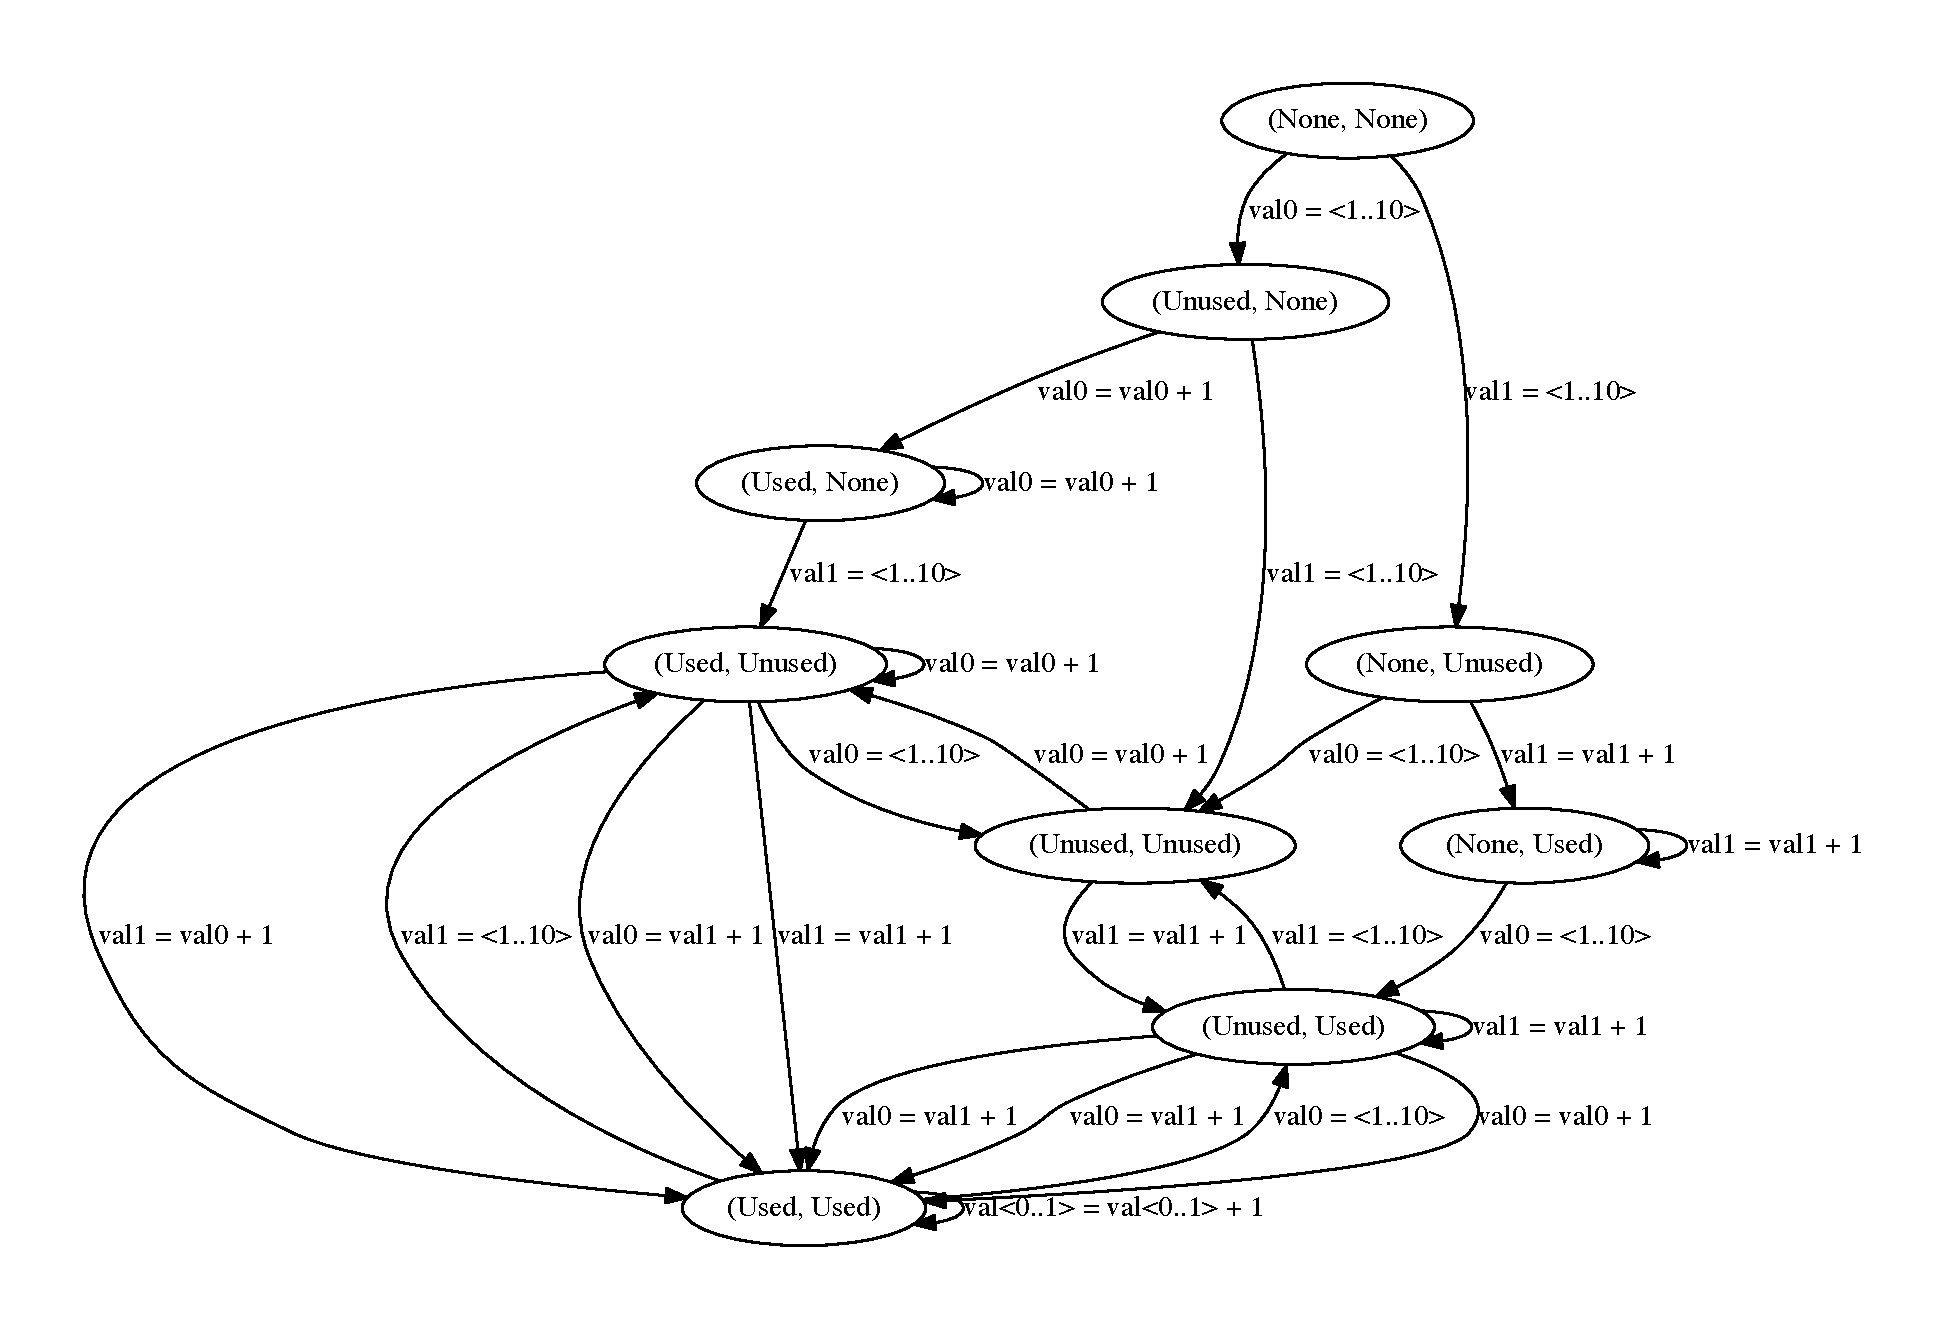
\includegraphics[width=\columnwidth]{states}
\caption{Constraints on actions in a test, based on pool states}
\label{fig:poolacts}
\end{figure}

{\scriptsize
\begin{code}
val0 = 1
val0 = 2 ...
val0 = 10
val1 = 1 ...
val1 = 10
\end{code}
}

From the initial state of the system, only these 20 actions are
\emph{enabled}.  \emph{Enabled} actions are those that can be executed in the
current state; the complete set of actions defined by a TSTL harness is always
finite, and the enabled set is always a subset of that finite set.  The first concept that is essential to understanding
TSTL semantics is that at any state of the
system, the only actions that are enabled are those that do not
\emph{use} any non-initialized pool values.  Any appearance of a pool
value is considered a \emph{use}, with the single exception of the left-hand-side of a
{\tt :=} initialization (not normal assignment)\footnote{The definition of
use is the only distinction between {\tt :=} and normal Python
assignment, and {\tt :=} is implemented as Python assignment, and appears
as such when test cases are printed.}.  The second concept is that a value
cannot be initialized (appear on the lhs of {\tt :]}) until after at
least one action
that uses it has been executed.  Figure \ref{fig:poolacts} shows the
consequences of these rules for the simple value assignment harness
above.  The nodes in the graph are labeled with {\tt state(val0),
  state(val1)}, where state is
either {\tt None} (uninitialized), {\tt Unused} (initialized
but never used) or {\tt Used} (initialized and used at least once).
Starting from the initial state {\tt (None, None)}, a valid test is any path
through the graph. 

Tests that can be produced by this harness include, therefore,
sequences like  {\tt val0 = 3; val0 = val0 + 1; val1 = 4; val1 = val0
  + 2} and {\tt val1 = 10; val0 = 6; val0 = val1 + 1; val0 = 2; val1 =
  15}.  However, {\tt val0 = val0 + 1; val0 = 2} and
{\tt val0 = 1; val1 = 1; val1 = 4} are not valid tests, because they
either use an uninitialized pool value, or re-initialize an unused
pool (a clearly useless action sequence).

\subsection{Other Core Language Features}

The example TSTL harness in Figure \ref{fig:MakeFeatureLayer} shows a
few other important core elements of TSTL.  First, choice templates
are not limited to integer ranges, but can include arbitrary items in
a list, e.g, {\tt <fc> := <["d1.shp", "d2.shp", "d3.shp"]>}.
Normally, when an action raises an uncaught exception, this is
considered a test failure.  Prefixing an action with a set of
exception names in curly braces (e.g., {\tt \{IOError\}}) indicates
that some exceptions are expected, and do not indicate a failure.
More critically, actions can be prefixed by arbitrary guards, using
the syntax {\tt guard -> action}.  The simple ArcPy harness chooses
field names for SQL by first extracting a list of all fields in some
feature class.  It then allows a field name to be chosen by taking the
name of the first field in the list.  However, since the harness also
allows the list of fields to be stepped through by discarding the
initial element, the name extraction has to be guarded to ensure that
tests won't try to extract names from an empty field list:  {\tt
  len(<fieldlist,1>) >= 1 -> <fieldname> := <fieldlist> [0].name}.
The {\tt <fieldlist,1>} construct, which can also be used outside of a
guard, indicates that this pool value should not be produced using
normal template expansion (instantiated as both {\tt fieldname0} and
{\tt fieldname1}) but rather than it should copy the comma indexed
appearance of that pool in each expansion (indexing starts from 1).  This makes sure the guard
is over the same pool value that is used in the action.

TSTL also supports post-conditions on actions, in the form {\tt action
  => post-condition}, where an assertion is
checked after certain actions are performed.  For example, because
some known ArcPy bugs involve addition of incorrect characters to
field names in a database, we could add code to check that all field
names in feature classes are correct.  TSTL supports {\tt init:} code
in the preamble, which is called before each test starts.  We can then
make sure that a library call to add a field to a feature class adds
it to a database of all field names collected at the start of testing,
and check the set of values returned by 
at the beginning of each test, and store these in a dictionary.  We
can update the data if, for example, we add a field, and then check
that all field names are correct every time we access a feature
classes' fields.  Ending a line in a backslash indicates the action
continues on the next line of the file.

{\scriptsize
\begin{code}
init: <fieldnames> = getAllFieldNames(getFeatureClasses())

\{ExecuteError\} not (<fc,1> in <hascursor>) -> \\
   AddField\_management(<fc>,<fieldname>,<fieldtype>); \\
   <fieldnames> [<fc,1>].add([<fieldname,1>])

\{IOError\} <fieldlist> := ListFields(<fc>) \\
  => sorted(<fieldlist,1>) == sorted(list(<fieldnames> [<fc,1>]))
\end{code}
}

Note the additional guard on adding fields --- we have discovered that
adding a field to a feature class that has any database cursors active
tends to crash ArcPy.  In post-conditions, the construct {\tt
  pre<(expr)>} allows access to values of expressions from before the
action is executed, as a further convenience.

When a correctness property is more general than a post-condition on a
single action, it can also be included in the preamble, to be checked
after every action.  Our field name property could therefore also be
stated as {\tt property: sorted(ListFields(<fc>)) ==
  sorted(list(<fieldnames> [<fc,1>]}.  The advantage is that this will
catch problems even if we never construct a {\tt fieldlist}; the
disadvantage is that testing slows to check all field names for all
feature classes, after every action.

Another useful feature of TSTL is the ability to create
\emph{reference} pools, where every action on pool values is mirrored
by an action on a reference version of that pool.  This makes it
possible to perform differential testing \cite{Differential} on a
per-pool basis, rather than at the whole-system level, allowing
complex partial specifications.  For example, in ArcPy we may want to
ensure that operations are deterministic: no GIS operations produce
different results, given the same underlying starting feature class
data.  Assuming in raw Python in the preamble we have defined {\tt
  identityFunction} as an identity function and {\tt copyFCName} as a
function that takes a feature class name and transforms it into a
generated name for a reference copy of the feature class, the
following mirrors all actions on feature classes on a reference copy,
and checks that the feature class and its reference always have the
same fields.

{\scriptsize
\begin{code}
pools:
  <basefc> 2 CONST
  <fc> 2 CONST REF

<basefc> := <[``d1.shp'', ``d2.shp'', ``d3.shp'']>; \\
  CopyFeatures\_management(<basefc,1>,copyFCName(<basefc,1>)
<fc> := identityFunction(<basefc>)
\{IOError\} <fieldlist> := ListFields(<fc>)

references:
  identityFunction ==> copyFCName

compares:
  ListFields
\end{code}
}

When instantiating the action templates, TSTL always produces a copy
of every action containing any reference pool values.  First, the pool
values are replaced with their reference copies; second, all the
syntactic transformations (which can include arbitrary Python regular
expressions) in the {\tt references} declaration are applied.
Finally, if any string matches a regular expression in a {\tt
  compares} declaration, the return values or assigned values in the
action are compared with those for the reference version.

\subsection{How to Build a TSTL Harness}

In the introduction, we noted that one problem with automatic
extraction of harnesses by tools is that in order to effectively test
complex systems, it is important to incrementally build testing
capability, understanding the effort as it increases in scope.  TSTL
naturally supports this methodology.  The ArcPy harness, though
complex, was developed by starting with a small number of ArcPy
functions, and determining their parameters.  These functions were
chosen because they were likely to expose faults easily.  Once
functions have been chosen, and their parameters are known,
developing a harness can often be a clean, iterative process:

\begin{enumerate}
\item Choose a new function (or set of related functions) to include
  in the harness.
\item Determine all parameters types.
\item If there is no pool that can produce these types, determine how
  to produce these types, and add pools and pool initialization actions for
  those pools.  This may require adding some additional
  functions (in which case, go to step 1 and start with those
  functions).
\item Add an action to call the function(s) being added.  If relevant,
  allow any expected exceptions, guards, and post-conditions to check.
\item Run testing, examine code coverage and failures to evaluate the
  added code, and repeat from step 1.
\end{enumerate}

These steps, combined with occasional refactoring or generalization of
parts of the harness, can effectively test even a large library, while
maintaining tester understanding and control.   In the ArcPy test
harness development, most of the effort was spent in this cycle, with
major exceptions being the implementation of a method allowing users
to provide their own GIS data on which testing is based, and effort to
improve the TSTL tool infrastructure to support testing a complex
application in a Windows environment.

\section{TSTL Tools}
\label{sec:tools}

The following tools are provided in the TSTL distribution on github \cite{tstl}.  Installing the TSTL module allows the compiler, called {\tt tstl}, to be used at the command line.  Other tools are included in the {\tt generators} and {\tt utilities} directories of the distribution as Python scripts.

\subsection{The TSTL Compiler}

Given a harness file defined in the language discussed above, the TSTL compiler generates a stand-alone Python class that allows testing of the SUT.  This generated code does not depend on the TSTL system being installed, only on any modules the testing itself uses, and on whether code coverage is requested.  By default, the compiler produces a class supporting code coverage using the {\tt coverage.py} module, and assumes this is installed.  The TSTL compiler also allows a user to control some fine-grained coverage measures (e.g, is coverage measured during initialization and module reloads?), and force a system to use replay-based backtracking by default.

\subsection{Test Generators}

TSTL comes with a complex, highly configurable, pure random tester (supporting numerous command-line options).  The included random tester provides a number of useful options, of which a subset are shown in Figure \ref{tab:rt}.   

\begin{figure}
{\scriptsize
\begin{itemize}
\item {\tt depth <int>}: Determines the length of generated tests.
\item {\tt timeout <int>}: Determines the maximum time spent generating tests, in seconds.
\item {\tt seed <int>}: Determines the random seed for testing.
\item {\tt maxTests <int>}: Determines the maximum number of tests to be generated.
\item {\tt running}: Produce on-the-fly, time-stamped code coverage information, for analyzing performance of testing algorithms. 
\item {\tt replayable}: Produce a log of the current test, so even it crashes Python the test can be reproduced, delta-debugged, made stand-alone, or otherwise analyzed.
\item {\tt total}: Produce a total log of all test activity, including across resets, for systems where reset is not complete (so tests across resets can be delta-debugged).
\item {\tt quickTests}:  Produce ``quick test'' files \cite{icst14}, each containing a minimal test to cover a set of branches of the SUT. 
\item {\tt normalize}: Apply additional, custom term-rewriting based simplifications of test cases that often further minimize delta-debugged test cases. 
\item {\tt generalize}: Apply generalization that elaborates each failing test with annotations showing similar tests that also fail. 
\item {\tt swarm:}  Apply swarm testing \cite{ISSTA12} to test generation.
\end{itemize}
}
\caption{Some options for the TSTL random test generator.}
\label{tab:rt}
\end{figure}

To our knowledge, TSTL's random tester is the first general-purpose random testing tool to incorporate the powerful swarm testing \cite{ISSTA12} algorithm, which has previously been used to test compilers \cite{ISSTA13,ZhendongPLDI14} and file systems.  TSTL's version of swarm testing is more sophisticated than previously published versions, in that it analyzes the dependency graph of TSTL actions to avoid producing degenerate test configurations, improving performance over naive swarm testing.  In addition to these stable, commonly used operations, the random tester includes novel experimental options, such as the ability to guide random testing by a user supplied Markov model or operational profile \cite{Hamlet94}.  TSTL makes implementing novel test generation methods simple, as discussed below.

The base TSTL tools also use the TSTL interface to support explicit-state model-checking \cite{ModelChecking,SPIN}, using either Depth-First-Search (DFS) or Breadth-First-Search (BFS) strategies.  TSTL uses Python's {\tt deepcopy} tools to provide a simple, easy to use interface for automatically storing and restoring pool states, making these algorithms trivial to implement.  There is no fundamental technical difference between performing (theoretically exhaustive) systematic searches of a well-defined transition system or random exploration.  Using the same transition system definition for both purposes has considerable advantages, as pointed out in previous work \cite{woda08}, especially for effectively infinite-state systems where random walks will never saturate and exhaustive searches will never complete.
TSTL can (unlike SPIN or most explicit-state model checkers) apply BFS or DFS search even to systems without support for backtracking.  TSTL's abstract interface to an SUT (transition system) can be configured to provide replay-based simulation of state storage and retrieval.  This is required when, for example, a library uses a C extension and so Python's {\tt deepcopy} does not allow full copying of the state of pool objects, or when the system has hidden global state that cannot be captured in a pool value.  While state storage and backtracking is usually faster than replay, we find that for some systems the opposite is true, particularly for shallow search depths (which are typical for BFS of a complex system).

TSTL also supports custom abstraction of pools.  If a pool is declared with an {\tt ABSTRACT} annotation, the function after the {\tt ABSTRACT} keyword can be used to abstract all values for state-matching purposes during exhaustive exploration methods.  The {\tt state} method returns the concrete state of the system, and applying the {\tt abstract} function to this state returns an abstract version of the state to be used in state matching.  The core of a BFS, for example, can be expressed quite simply, irrespective of whether the system is using state storage and backtracking or replay (or has an abstraction or not) as:

{\scriptsize 
\begin{code}
old = sut.state()
for act in sut.enabled():
   sut.safely(act)
   new = sut.state()
   \# repr produces a hashable string representation
   absNew = repr(sut.abstract(new))
   if absNew not in visited:
      queue.append(new)
      visited[absNew] = True
      ...
   sut.backtrack(old)
\end{code}
}

This loop iterates through all enabled actions from the current state, and adds any not previously visited to the search queue.  Similar code works as the core of a DFS.  While not required for any of our testing efforts thus far, encoding temporal logic checking is also simple.  A B\"uchi automata can be encoded in Python, querying the SUT state and action choices to determine transitions.  Composing this with the SUT state is trivial.  We managed to implement the well-known nested DFS algorithm \cite{DoubleDFS} in less than 40 lines of code, taking the property automata as a tuple input {\tt(initial, trans, accept)}, where {\tt trans: (state, action, sut state) -> state}.

\subsection{Utilities for Test Case Manipulation}

TSTL provides the tools {\tt sandboxreducer} and {\tt standalone} for manipulating saved test cases produced by the random tester or the simple model checkers.  These were developed as part of the ArcPy testing process.  ArcPy faults tend to crash the system (this is also the reason the {\tt total} option was introduced), and thus cannot be simplified for debugging inside the test generator.   The sandbox reducer takes a testing log and, using subprocesses to handle crashes, produces delta-debugged and normalized test cases. It is also useful to report failing tests not as TSTL's internal test file format, but as standalone Python programs that cause a failure.  The {\tt standalone} utility takes a test log or a saved test case and produces a complete, stand-alone Python program that requires neither the generated TSTL interface nor any other TSTL tools.

\begin{figure}
{\scriptsize
\begin{code}
import sut
import glob

sut = sut.sut()

failed = 0
total = 0

for testFile in glob('regressions\\*.test'):
   t = sut.loadTest(testFile)
   total += 1
   if sut.failsAny(t):
       failed += 1
       print testFile,'FAILED:',sut.failure()

print total,'TESTS EXECUTED'
print failed,'TESTS FAILED'

print len(sut.allBranches()),'BRANCHES COVERED'
print len(sut.allStatements()),'STATEMENTS COVERED'
print sut.report('coverage.txt'),'\% STATEMENTS COVERED'
\end{code}
}
\caption{A small script to run stored regression tests}
\label{fig:regress}
\end{figure}


However, use of these tools is often not required.  Figure \ref{fig:regress} shows a simple, but complete, Python script for running regression tests generated using TSTL for a system.  This script examines the {\tt regressions} directory, replays each test in the directory, and reports on failing tests and code coverage.  Such a script can easily be customized to provide different tests for different budgets (e.g., prioritized by time, coverage, or to execute coverage-based 'quick tests').

\subsubsection{ArcPy Regression Generation}

One difficulty for ArcPy users is ensuring that their existing scripts
and tools work on new versions of ArcGIS.  Each recent major release
(10.2 and 10.3) after ArcPy's introduction has potentially included some changes
in the behavior of API calls.  Detecting when such changes cause a
script to break is difficult.  A first step would be an automatic way
to find when the return values for calls differ between ArcPy
versions.
Because installing multiple versions of ArcGIS on the same system is
difficult or impossible, our method for finding differences relies on
choosing a reference version (10.3 in our current efforts), and
generating a set of standalone tests that 1) cover a large amount of
ArcPy functionality, including invalid inputs to functions and 2)
record the return values and exceptions raised by calls.  These tests
can be run on any ArcPy version, and will report differences between
the tests and version 10.3.  Performing this kind of differential
testing \cite{Differential} on old or new major releases, or across 64
bit and 32 bit versions, is easy.  In the long run, we also want to
enable TSTL to produce Python 3.0+ code, for use with ArcGIS Pro,
which uses Python 3.4 instead of 2.7.  This has motivated a branch to
TSTL to support Python 3.0 (unfortunately, Python 3.0 is not fully
backwards compatible with earlier versions, and Python 2.7 is still
the most widely used Python, and non-pro versions of ArcPy only work
with 2.7).

We generate coverage-based regression tests using an approach called \emph{quick
  testing} \cite{icst14,stvrcausereduce}, which takes a set of tests
produced by random testing, and applies a test case reduction
algorithm \cite{DD} to produce smaller tests that have the same code
coverage as the very large, highly redundant, original set of test
cases.  Automatic quick-testing was added to TSTL's random test
generator to support ArcPy testing.  Combined with standalone test
generation, this allows us to produce test cases that can be run on
any version of ArcPy, and explore a large variety of behavior of the
code.  With ArcPy, coverage alone, unlike previous quick testing
efforts, is insufficient to ensure a useful regression test.  Because
coverage only considers the Python behavior of ArcPy (since we do not
have access to the source for the ArcGIS engine), it may group
behaviors that are not similar together.  We added the ability to
combine coverage preservation with preservation of all ArcPy messages
indicating a successful GIS engine operation, after abstracting away
such details as the runtime of the operation, and so forth.

However, just producing these coverage-and-engine-behavior preserving
standalone tests is not sufficient for good version comparison, since
standalone test cases as produced only check for properties defined in TSTL.  An
additional option was added to the standalone test generator, allowing
it to record the actual return values of all calls, the set of
exceptions thrown, the success/failure messages from the ArcPy engine, and so forth to more precisely record a test's
behavior on an ArcPy version.


\subsection{Visualization of Action Spaces}

\begin{figure}
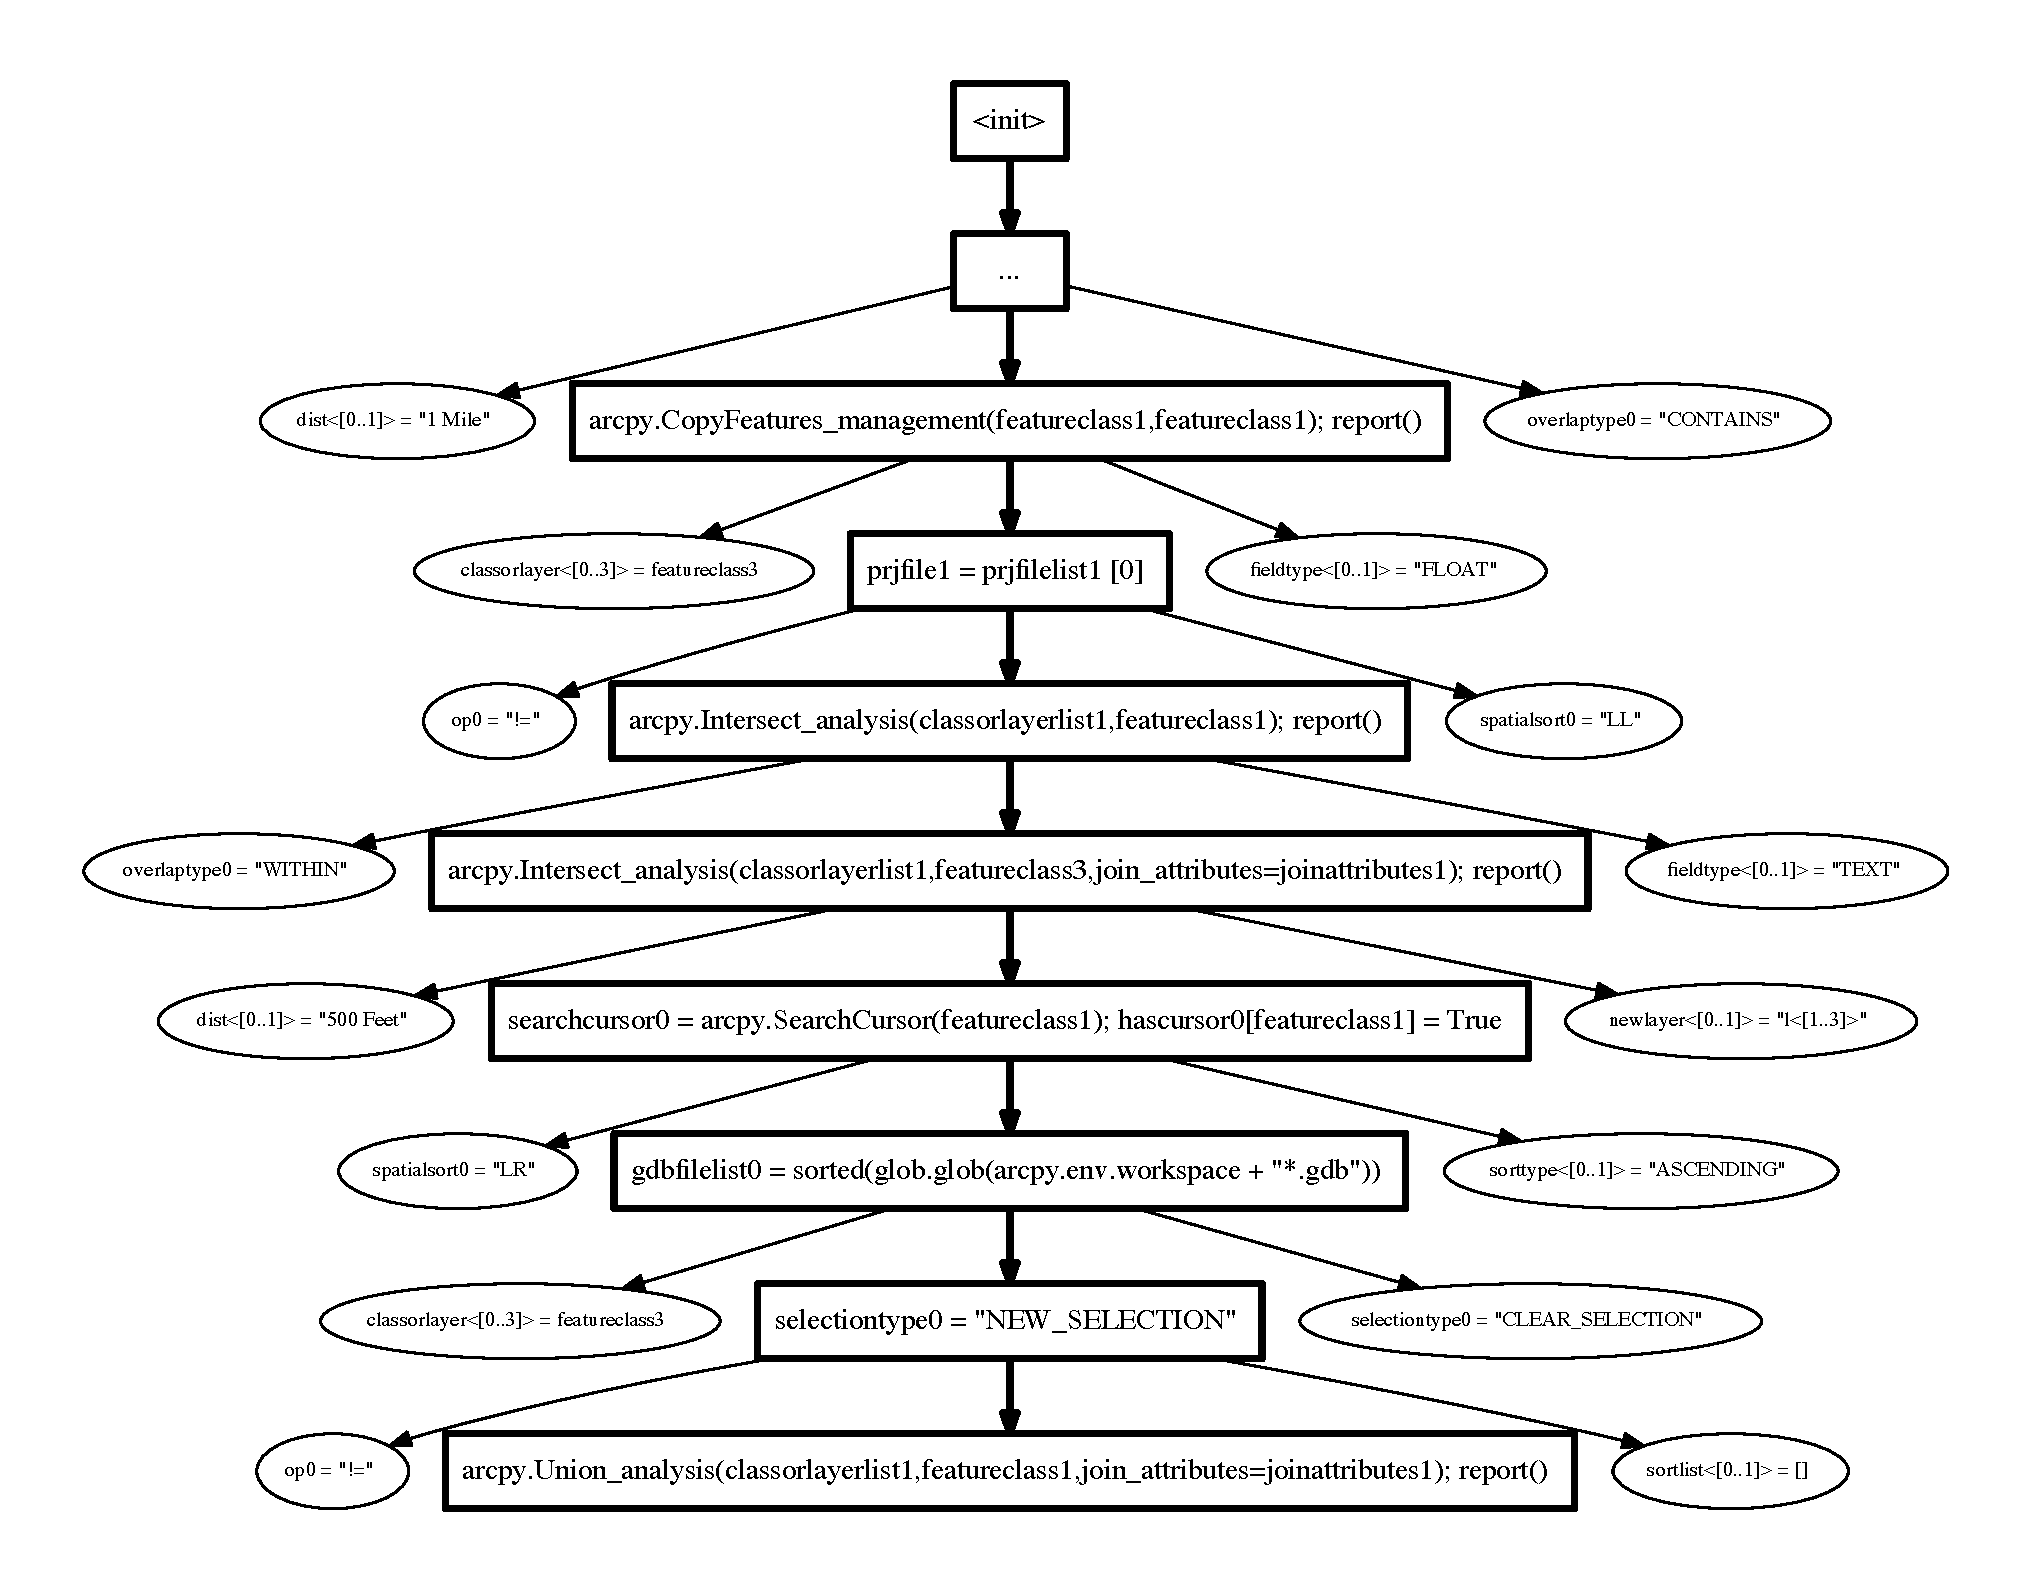
\includegraphics[width=\columnwidth]{shortgraph}
\caption{Start depth 20, depth 8, width 3 trace visualization for ArcPy testing.}
\label{fig:actions}
\end{figure}

Understanding the structure of the action graph produced by even a relatively simple TSTL harness can be difficult.  The structure is often infinite, and even in cases where there is a finite state space (perhaps introduced by abstraction) the graph is usually far too large for a convenient display.  However, we have found that a visual representation of typical trajectories through the system can be very helpful for understanding a complex test system.  The {\tt makegraph} utility takes as input a number of traces to produce, a starting depth, additional depth, and a test width.  It then produces in pdf form a number of graphs for traces like the one shown in Figure \ref{fig:actions}.  These trace graphs show, in bold, the actual action sequence chosen by a pure random tester, starting after a number of actions not shown (represented by the ``...'' node) and continuing up to the depth limit.  In addition to the actions taken, the graph also shows a random subset of additional enabled actions, with each step showing a number of actions equal to the width.  Because many actions are extremely similar, the graphing utility also summarizes actions that are the same, except for pool choice or integer constant, using the {\tt <[i..j]>} notation of TSTL.

\subsection{Building Your Own Testing Tools in TSTL}
\label{sec:build}

Describing the full interface provided by TSTL for use in testing tools is beyond the scope of this paper.  However, examining the source code of the included testers can provide a good starting point.  Implementing new test case manipulations usually involves understanding TSTL internal structures and how tests are stored.  Implementing novel test generation algorithms can often rely on just a handful of methods, shown in Figure \ref{methods} (there are many more methods for e..g, code coverage, but this minimal set can implement many test generation algorithms).

\begin{figure}
{\scriptsize
\begin{itemize}
\item {\bf restart():}  resets the system state and aborts the current test. 
\item {\bf test():} returns the current test.
\item {\bf replay(test):} replays a test, and returns a Boolean indicating success or failure of the test.
\item {\bf enabled():} returns a list of all currently enabled actions.
\item {\bf randomEnabled(random):}  given a Python random number generator object, returns a random enabled action, efficiently (avoiding unnecessary guard evaluations).
\item {\bf safely(action):} performs action (usually changing SUT state)  and returns a Boolean indicating whether the action performed raised any uncaught exceptions. 
\item {\bf check():} returns a Boolean indicating whether any properties fail for the current state.
\item {\bf error():} returns either {\tt None} (no error for the last action or {\tt check}), or a Python object representing an uncaught exception or failed property's backtrace.
\item {\bf state():} returns the current SUT state, as a set of values for all pools; for systems where state cannot be restored by pool values, or {\tt deepcopy} does not work, returns the current test.
\item {\bf backtrack(state):} takes a state or test produced by {\tt state} and restores the system to it.
\item {\bf allBranches():} returns the set of branches covered during all testing.
\item {\bf newBranches():} returns the set of branches covered during the last action executed that had not previously been covered.
\item {\bf currBranches():} returns the set of branches covered during the current test.
\item {\bf saveTest(test, filename):} saves a test in a file.
\item {\bf loadTest(filename):} loads a test from a file (and returns that test as the function's return value).
\end{itemize} 
}
\caption{Some core methods for testing an SUT.}
\label{methods}
\end{figure}

For example, a researcher aware of the literature showing that for many systems it is difficult to outperform random testing, due to its very low overhead \cite{ISSRE12,ISSTA12}, may consider simple modifications of random testing that do not greatly increase overhead.  One such example, with implementation, is shown in the original TSTL paper \cite{NFM15}.  We present another here.  Since the focus of this paper is on showing how to use TSTL, not novel test generation methods, we leave a complete development and statistically valid evaluation of our proposed approach to future work, but discuss briefly how to go about prototyping and evaluation using TSTL.

The idea is to perform random testing, but keep the final state of tests with unusually high coverage as potential starting points for future tests, potentially extending them far beyond the normal test length limit.  The approach is parameterized by {\tt MEMORY}, the number of ``good'' tests to store, by {\tt PEXTEND}, the probability of choosing to extend a ``good'' test rather than start a new test, by the {\tt TEST\_LENGTH} and by a {\tt TIMEOUT} parameter.  Leaving out imports and other boilerplate, the entire implementation is shown in Figure \ref{fig:keepgood}.

\begin{figure}
{\scriptsize
\begin{code}
goodTests = []
startTime = time.time()
while (time.time() - startTime <= TIMEOUT):
   if (len(goodTests) > 0) and (rgen.random() < PEXTEND):
     sut.backtrack(rgen.choice(goodTests)[1])
   else:
     sut.restart()
   for s in xrange(0,TEST\_LENGTH): 
      action = sut.randomEnabled(rgen)
      r = sut.safely(action)
      if len(sut.newBranches()) > 0:
         print time.time(),len(sut.allBranches()),'NEW BRANCHES:', sut.newBranches()
   if MEMORY > 0:
      goodTests.append((sut.currBranches(), sut.state()))
      goodTests = sorted(goodTests, reverse=True)[:MEMORY]
\end{code}
}
\caption{Implementing a very simple novel testing algorithm.}
\label{fig:keepgood}
\end{figure}

The implementation is trivial, relying only on the TSTL API and some very simple Python tools (sorting with automatic lexical ordering, time library, etc.).  We omit handling of failed tests, assuming the goal of this algorithm is simply to improve code coverage in fault-free systems for experimental evaluation.  This simple tool can be applied to any TSTL harness and will produce output showing when, in time, new branches were covered by the system.  This data can be used to produce Average-Percent-Branches-Detected (APBD) values and discovery curves \cite{issta14,Rothermel1999,rothermel01oct}. Comparison with simple random testing is easy, since setting {\tt MEMORY} to 0 gives pure memoryless random testing (alternatively, to avoid the overhead of the comparisons with 0, a dedicated version for random testing can be written).  A major threat to validity in many comparisons of testing or explicit-state model checking algorithms is that different underlying infrastructure for different algorithms may end up outweighing even moderately sized effects due to the underlying algorithms.  With TSTL, fair comparisons are much easier, since the TSTL interface does most of the computational work that is common to multiple algorithms, with the same overhead.  Evaluating an algorithm can be as simple as finding a large number of suitable programs without failures (or where failures don't make coverage values invalid) and performing enough trials to establish statistical validity for comparisons with APBD values for known algorithms.  Evaluation in terms of discovered faults or time-until-discovery of a fault is nearly as simple.  This algorithm is of some interest, in that while it requires backtracking, the frequency of backtracking is low enough to be potentially applicable even to systems like ArcPy where backtracking is only possible via expensive test replay.  While a mature version of this method would require many SUTs and experiments, as well as investigation of suitable values for {\tt MEMORY} and {\tt PEXTEND}, Figure \ref{fig:compare} shows that average branch discovery curves for ArcPy can sometimes be improved, even using the  arbitrarily chosen parameters of a size 5 memory and a 20\% probability of using a ``good'' test as a starting point.  The simplicity of the Python implementation makes performing automatic experiments with different parameters and test lengths trivial.  Experiments can also take advantage of Python libraries for automatic statistical analysis and plotting of results.

\begin{figure}
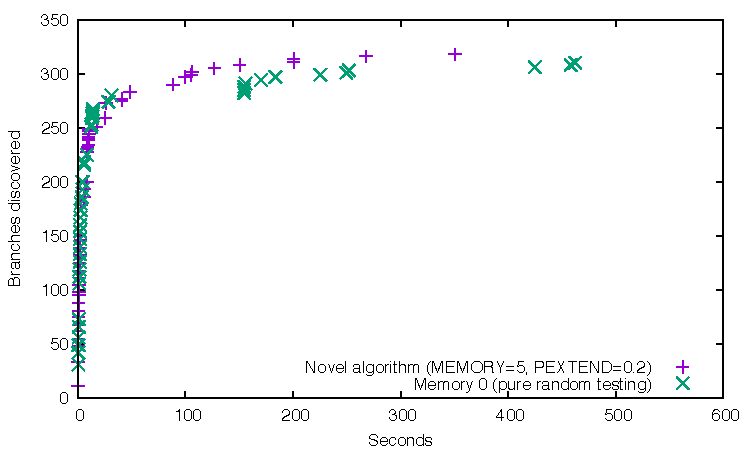
\includegraphics[width=\columnwidth]{memory}
\caption{Comparing branch coverage for 10 minute runs of two test generation methods.}
\label{fig:compare}
\end{figure}

\section{TSTL as a Testing Library Generator}
\label{sec:langext}

While TSTL is easily used as ``just another tool'' that allows testing of an SUT, and a construction kit to build your own testing tools, TSTL can also be understood as a generator of libraries.  ArcPy is a site package that makes it easy to perform GIS tasks using Python.  NumPy \cite{NumPy} and SciPy \cite{SciPy} are libraries that make performing scientific computing tasks easy with Python.  QIIME \cite{QIIME}, Biopython \cite{biopython}, and scikit-bio \cite{scikitbio} are libraries that make performing bioinformatics tasks easy using Python.  

\section{Faults Discovered Using TSTL}

\subsection{ArcPy Faults}

\begin{figure}
{\scriptsize 
\begin{code}
shapefilelist0 = glob.glob("C:\\Arctmp\\*.shp")                             \textcolor{black!60}{\# STEP 0}
\textcolor{black!60}{\#[}
shapefile0 = shapefilelist0 [0]                                           \textcolor{black!60}{\# STEP 1}
newlayer0 = "l1"                                                          \textcolor{black!60}{\# STEP 2}
\textcolor{black!60}{\#  or newlayer0 = "l2" }
\textcolor{black!60}{\#  or newlayer0 = "l3" }
\textcolor{black!60}{\#  swaps with steps 3 4 5 6 7}
\textcolor{black!60}{\#] (steps in [] can be in any order)}
\textcolor{black!60}{\#[}
featureclass0 = shapefile0                                                \textcolor{black!60}{\# STEP 3}
\textcolor{black!60}{\#  swaps with step 2}
fieldname0 = "newf1"                                                      \textcolor{black!60}{\# STEP 4}
\textcolor{black!60}{\#  or fieldname0 = "newf2" }
\textcolor{black!60}{\#  or fieldname0 = "newf3" }
\textcolor{black!60}{\#  swaps with steps 2 8}
selectiontype0 = "SWITCH\_SELECTION"                                       \textcolor{black!60}{\# STEP 5}
\textcolor{black!60}{\#  or selectiontype0 = "NEW\_SELECTION" }
\textcolor{black!60}{\#  or selectiontype0 = "ADD\_TO\_SELECTION" }
\textcolor{black!60}{\#  or selectiontype0 = "REMOVE\_FROM\_SELECTION"}
\textcolor{black!60}{\#  or selectiontype0 = "SUBSET\_SELECTION"}
\textcolor{black!60}{\#  or selectiontype0 = "CLEAR\_SELECTION"   }
\textcolor{black!60}{\#  swaps with steps 2 8}
op0 = ">"                                                                 \textcolor{black!60}{\# STEP 6}
\textcolor{black!60}{\#  or op0 = "<" }
\textcolor{black!60}{\#  swaps with steps 2 8}
val0 = "100"                                                              \textcolor{black!60}{\# STEP 7}
\textcolor{black!60}{\#  or val0 = "1000" }
\textcolor{black!60}{\#  swaps with steps 2 8}
\textcolor{black!60}{\#] (steps in [] can be in any order)}
arcpy.MakeFeatureLayer\_management(featureclass0, newlayer0)               \textcolor{black!60}{\# STEP 8}
\textcolor{black!60}{\#  swaps with steps 4 5 6 7}
arcpy.SelectLayerByAttribute\_management(newlayer0,selectiontype0,
   ' "'+fieldname0+'" '+op0+val0)                                         \textcolor{black!60}{\# STEP 9}
arcpy.Delete\_management(featureclass0)                                    \textcolor{black!60}{\# STEP 10}
arcpy.SelectLayerByAttribute\_management(newlayer0,selectiontype0,
   ' "'+ fieldname0+'" '+op0+val0)                                        \textcolor{black!60}{\# STEP 11}
\end{code}
}
\caption{Deleting a feature class does not invalidate or delete layers that depend on it.}
\label{fault1}
\end{figure}

In the process of testing ArcPy with TSTL, we discovered six faults
(thus far) that can cause an ArcPy script to crash.  While we have (as
discussed in the language section) some properties that also check for
data corruption and determinism of GIS analysis, we are not focusing
on these until we have a reliable way to avoid system crashes.   In
order to give an idea of what TSTL test cases look like, we discuss
briefly one of these ArcPy crashes.

ArcPy crashes when the feature class from which a layer is produced is
deleted, and the layer is used in a {\tt SelectLayer} call (this
version shows an attribute-based selection, but location selection
will cause the same problem): (Figure \ref{fault1}).  The underlying issue seems to be that
while operations on a deleted feature class properly notify a user the
feature class does not exist, ArcPy or ArcGIS does not track that
layers produced from a feature class should also be deleted/invalidated
when the feature class is deleted.  Layers are not copies
of a feature class, but essentially new \emph{views} of a feature class.
This means that when the underlying feature class is modified or
deleted, the view needs to be updated to reflect that change, and this
is not correctly implemented.  Figure \ref{fault1} shows part of an
annotated, reduced, normalized, and generalized test stand-alone test
case (with the boilerplate, function definitions, and imports
removed) for this fault.  The final line of code crashes ArcPy and the
Python interpreter.  Comments indicate alternative similar tests that
also fail.  In this case, TSTL's additional reduction steps (based on
term rewriting in the action language) remove almost half the steps in
the original, delta-debugged test case.

\subsection{Faults in Other Systems}

TSTL has is only slightly over a year old.  However, students using
TSTL in graduate classes on software testing have already, with
minimal assistance, discovered faults in some real-world systems.  Not
all of these are confirmed and reported yet.

First, TSTL testing revealed a fault in either the widely-used {\tt
  PyOpenCL} library, the even more widely-used {\tt OpenCL}
infrastructure, or (possibly) the NVIDIA hardware being used.  We are
still investigating this problem, but it appears to be a genuine
fault, though debugging and assigning blame is complex due to the
layers of software involved.  Second, TSTL testing found cases where distance metrics that were supposed to
be symmetric in the popular fuzzy-string-matching library FuzzyWuzzy.
Third, TSTL testing revealed numerous problems with the {\tt
  astropy.table} module of the AstroPy
library, used by many professional astronomers and astrophysicists.
Finally, TSTL has been used to discover faults in the TSTL API itself.

\section{Related Work}

This work builds on the idea behind delta-debugging \cite{DD}: tests should not contain extraneous information that is not needed to
reproduce failure (or some other behavior \cite{icst2014,stvrcausereduce}).  Delta-debugging and slicing
\cite{TCminim} are limited, generally, to producing subsets of the
original test, not modifying parts of the test to obtain further
simplicity.  We extend this concept by also allowing modification or
re-ordering, which also allows further length reduction.

%Some earlier work in bounded model checking modified counterexamples to use
%numerically smaller values \cite{MakeMost} but otherwise did not aim
%to simplify or normalize failures.

Normalization is in part motivated by the fuzzer taming \cite{PLDI13}
problem: determining how many distinct faults are present in a large
set of failing tests.  This is a key problem in practical
application of automated testing.  Previous work on fuzzer taming
\cite{PLDI13} used delta-debugging to reduce some tests to
syntactic duplicates.

Zhang \cite{SaiSimple} proposed an alternative approach to semantic
test simplification that, like our approach, is able to modify, rather
than simply remove, portions of a test.  However, because Zhang
operates directly over a fragment of the Java language, rather than
using an abstraction of test actions allowed, the set of rewrite
operations performed is highly restricted: no new methods can be
invoked, statements cannot be re-ordered, and no new values are used.
These restrictions limit the approach's ability to simplify tests and
make it inappropriate for  normalization, as opposed to simplification.  The approach also performs little
syntactic normalization: e.g., it does not even force a test to use
fixed variable names when variable name is irrelevant.  CReduce
\cite{CReduce} performs some simple normalization as part of a complex
test reduction scheme for C code, and the peephole-rewrite scheme
used in CReduce is also an inspiration for the approach taken by our
normalizer.

Work on automatically producing readable tests \cite{Guava,Readable} is also
related, in that it aims to ``simplify'' tests.  Readable tests are
intended to assist debugging by humans, while our
normalization and generalization aims to increase the information
density of a test, further reduce length, and address the fuzzer taming problem.  The approaches are
orthogonal and could likely be profitably combined: users might be
best served by normalized, generalized tests modified to improve readability.

The most closely related work to our generalization efforts is Pike's
SmartCheck \cite{SmartCheck}.  SmartCheck targets algebraic data in
Haskell, and offers an interesting alternative approach to reduction
and generalization.  Test generalization is also akin to dynamic invariant generation,
in that it informs the user of invariants over a series of test
executions \cite{Daikon}.  The only other work we are aware of that is
similar to generalization concerns essential and accidental aspects of
model checking counterexamples \cite{FreeWill,MakeMost,SPIN03}.  

\bibliographystyle{spmpsci}      % mathematics and physical sciences
%\bibliographystyle{spphys}       % APS-like style for physics
\bibliography{bibliography}   % name your BibTeX data base



\end{document}
% end of file template.tex

